\begin{bt}%[9D6H18-2]
% nguon: Cụm 10 – Đề tham khảo Tuyển sinh 10 năm học 2026-2027 TP.HCM – Đề số 28
Cho hàm số $y = \dfrac{x^2}{3}$ có đồ thị là parabol $(P)$.
\begin{enumerate}[a)]
    \item Vẽ đồ thị $(P)$ trên mặt phẳng tọa độ $Oxy$.
    \item Tìm tọa độ các điểm thuộc $(P)$ (khác gốc tọa độ) có tung độ gấp hai lần hoành độ.
\end{enumerate}
\loigiai{
\begin{enumerate}[a)]
    \item Bảng giá trị:
    \begin{center}
    \begin{tabular}{|c|c|c|c|c|c|}
    \hline
    $x$ & $-3$ & $-1{,}5$ & $0$ & $1{,}5$ & $3$ \\ \hline
    $y = \dfrac{x^2}{3}$ & $3$ & $0{,}75$ & $0$ & $0{,}75$ & $3$ \\ \hline
    \end{tabular}
    \end{center}
    Đồ thị parabol $(P)$ đi qua gốc tọa độ $O(0;0)$ và các điểm $(-3;3)$, $(-1{,}5; 0{,}75)$, $(1{,}5; 0{,}75)$, $(3;3)$.
    \begin{center}
    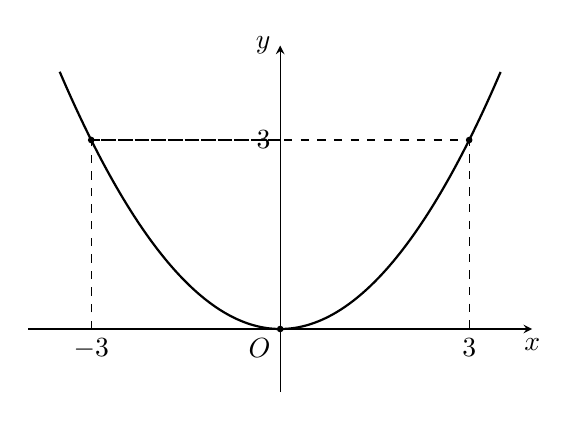
\begin{tikzpicture}[>=stealth,scale=0.8]
        \draw[->] (-4,0) -- (4,0) node[below] {$x$};
        \draw[->] (0,-1) -- (0,4.5) node[left] {$y$};
        \node[below left] at (0,0) {$O$};
        \draw[dashed] (-3,0) node[below] {$-3$} -- (-3,3) -- (3,3) -- (3,0) node[below] {$3$};
        \draw[dashed] (-3,3) -- (0,3) node[left] {$3$};
        \draw[thick,smooth,samples=100,domain=-3.5:3.5] plot(\x,{(1/3)*(\x)^2});
        \fill (-3,3) circle (1.5pt) (0,0) circle (1.5pt) (3,3) circle (1.5pt);
    \end{tikzpicture}
    \end{center}
    \item Điểm thuộc $(P)$ có tung độ gấp hai lần hoành độ nên thỏa mãn $y = 2x$.\\
    Ta có phương trình hoành độ giao điểm:
    $$\dfrac{x^2}{3} = 2x \iff x^2 - 6x = 0 \iff x(x - 6) = 0 \iff \left[\begin{aligned} &x = 0\text{ (loại vì khác gốc tọa độ)} \\ &x = 6\text{ (nhận)}. \end{aligned}\right.$$
    Với $x = 6 \implies y = 2 \cdot 6 = 12$.\\
    Vậy tọa độ điểm cần tìm là $(6; 12)$.
\end{enumerate}
}
\end{bt}

\begin{bt}%[9D6H20-2]
% nguon: Cụm 10 – Đề tham khảo Tuyển sinh 10 năm học 2026-2027 TP.HCM – Đề số 28
Cho phương trình $x^2 - 9x + 2 = 0$ có hai nghiệm $x_1, x_2$. Không giải phương trình, hãy tính giá trị biểu thức:
$$A = \dfrac{x_1^2}{2} - \left(\dfrac{x_1 - x_2^2}{2} - \dfrac{1}{x_2}\right).$$
\loigiai{
Phương trình $x^2 - 9x + 2 = 0$ có:
$$\Delta = (-9)^2 - 4 \cdot 1 \cdot 2 = 81 - 8 = 73 > 0.$$
Do $\Delta > 0$ nên phương trình có hai nghiệm phân biệt $x_1, x_2$.\\
Theo định lý Vi-ét, ta có:
$$\begin{cases} x_1 + x_2 = 9 \\ x_1 x_2 = 2. \end{cases}$$
Ta có $x_1^2 + x_2^2 = (x_1 + x_2)^2 - 2x_1 x_2 = 9^2 - 2 \cdot 2 = 81 - 4 = 77$.\\
Biến đổi biểu thức $A$:
$$A = \dfrac{x_1^2}{2} - \dfrac{x_1 - x_2^2}{2} + \dfrac{1}{x_2} = \dfrac{x_1^2 + x_2^2 - x_1}{2} + \dfrac{1}{x_2} = \dfrac{x_1^2 + x_2^2}{2} - \dfrac{x_1}{2} + \dfrac{1}{x_2} = \dfrac{x_1^2 + x_2^2}{2} - \dfrac{x_1 x_2 - 2}{2x_2}.$$
Thay $x_1^2 + x_2^2 = 77$ và $x_1 x_2 = 2$ vào biểu thức $A$, ta được:
$$A = \dfrac{77}{2} - \dfrac{2 - 2}{2x_2} = \dfrac{77}{2}.$$
}
\end{bt}

\begin{bt}%[9D8H26-3]
% nguon: Cụm 10 – Đề tham khảo Tuyển sinh 10 năm học 2026-2027 TP.HCM – Đề số 28
Người ta thống kê các loại ô tô chạy qua một trạm thu phí trong một giờ và thu được số liệu sau:
\begin{center}
\begin{tabular}{|l|c|c|c|c|}
\hline
\textbf{Loại xe} & Xe $4$ chỗ & Xe $7$ chỗ & Xe $9$ chỗ & Xe từ $16$ chỗ trở lên \\ \hline
\textbf{Số lượng xe} & $9$ & $14$ & $5$ & $3$ \\ \hline
\end{tabular}
\end{center}
\begin{enumerate}[a)]
    \item Tính tổng số xe qua trạm thu phí trong $1$ giờ đó.
    \item Tính xác suất của biến cố $A$: ``Xe qua trạm là xe $4$ chỗ''.
    \item Tính xác suất của biến cố $B$: ``Xe qua trạm là xe dưới $9$ chỗ''.
\end{enumerate}
\loigiai{
\begin{enumerate}[a)]
    \item Tổng số xe qua trạm trong $1$ giờ là:
    $$9 + 14 + 5 + 3 = 31\text{ (xe)}.$$
    \item Không gian mẫu có $n(\Omega) = 31$.\\
    Số kết quả thuận lợi cho biến cố $A$ (xe $4$ chỗ) là: $n(A) = 9$.\\
    Xác suất của biến cố $A$ là:
    $$P(A) = \dfrac{n(A)}{n(\Omega)} = \dfrac{9}{31}.$$
    \item Các loại xe dưới $9$ chỗ gồm xe $4$ chỗ và xe $7$ chỗ.\\
    Số kết quả thuận lợi cho biến cố $B$ là:
    $$n(B) = 9 + 14 = 23.$$
    Xác suất của biến cố $B$ là:
    $$P(B) = \dfrac{n(B)}{n(\Omega)} = \dfrac{23}{31}.$$
\end{enumerate}
}
\end{bt}

\begin{bt}%[9D6V21-3]
% nguon: Cụm 10 – Đề tham khảo Tuyển sinh 10 năm học 2026-2027 TP.HCM – Đề số 28
Một mảnh vườn hình chữ nhật có chiều dài $25\text{ m}$, chiều rộng bằng $\dfrac{3}{5}$ chiều dài. Người ta làm hai lối đi trong vườn: một lối đi dọc rộng $x\text{ (m)}$ và một lối đi ngang rộng $2x\text{ (m)}$. Phần đất còn lại dùng để trồng cây.
\begin{enumerate}[a)]
    \item Viết biểu thức theo $x$ biểu thị diện tích đất dùng để trồng cây.
    \item Biết rằng diện tích lối đi lớn hơn diện tích đất trồng cây là $175\text{ m}^2$. Tìm $x$.
\end{enumerate}
\loigiai{
\begin{enumerate}[a)]
    \item Chiều rộng của mảnh vườn là:
    $$25 \cdot \dfrac{3}{5} = 15\text{ (m)}.$$
    Diện tích toàn bộ mảnh vườn là:
    $$S_{\text{vườn}} = 25 \cdot 15 = 375\text{ (m}^2\text{)}.$$
    Phần đất còn lại dùng để trồng cây có chiều dài là $25 - x\text{ (m)}$ và chiều rộng là $15 - 2x\text{ (m)}$.\\
    Biểu thức diện tích đất trồng cây là:
    $$S_{\text{cây}} = (25 - x)(15 - 2x)\text{ (m}^2\text{)}.$$
    \item Điều kiện của $x$: $\begin{cases} x > 0 \\ 15 - 2x > 0 \end{cases} \implies 0 < x < 7{,}5$.\\
    Diện tích của hai lối đi là:
    $$S_{\text{lối}} = S_{\text{vườn}} - S_{\text{cây}} = 375 - (25 - x)(15 - 2x)\text{ (m}^2\text{)}.$$
    Theo đề bài, diện tích lối đi lớn hơn diện tích đất trồng cây là $175\text{ m}^2$, nên ta có phương trình:
    $$\big[375 - (25 - x)(15 - 2x)\big] - (25 - x)(15 - 2x) = 175$$
    $$\iff 375 - 2(25 - x)(15 - 2x) = 175$$
    $$\iff 2(25 - x)(15 - 2x) = 200 \iff (25 - x)(15 - 2x) = 100$$
    $$\iff 375 - 50x - 15x + 2x^2 = 100 \iff 2x^2 - 65x + 275 = 0.$$
    Ta có $\Delta = (-65)^2 - 4 \cdot 2 \cdot 275 = 4225 - 2200 = 2025 > 0$, $\sqrt{\Delta} = 45$.\\
    Phương trình có hai nghiệm:
    $$x_1 = \dfrac{65 - 45}{4} = 5\text{ (thỏa mãn } 0 < x < 7{,}5\text{)},$$
    $$x_2 = \dfrac{65 + 45}{4} = 27{,}5\text{ (loại)}.$$
    Vậy $x = 5\text{ m}$.
\end{enumerate}
}
\end{bt}

\begin{bt}%[9H0V31-3]
% nguon: Cụm 10 – Đề tham khảo Tuyển sinh 10 năm học 2026-2027 TP.HCM – Đề số 28
Một cái bình hình trụ có bán kính đáy là $4\text{ cm}$ và chiều cao là $16\text{ cm}$.
\begin{enumerate}[a)]
    \item Tính thể tích nước cần đổ vào để mực nước trong bình cao $14\text{ cm}$, biết lúc đầu bình không chứa nước.
    \item Người ta có một số viên bi thủy tinh hình cầu cùng đường kính là $1{,}6\text{ cm}$. Có thể thả chìm vào nước nhiều nhất bao nhiêu viên bi để nước trong bình không bị tràn ra ngoài?
\end{enumerate}
Biết thể tích hình trụ là $V = \pi R^2 h$ ($R$ là bán kính đáy, $h$ là chiều cao) và thể tích hình cầu là $V = \dfrac{4}{3}\pi r^3$ ($r$ là bán kính).
\loigiai{
\begin{enumerate}[a)]
    \item Thể tích nước cần đổ vào để mực nước cao $14\text{ cm}$ là:
    $$V_1 = \pi R^2 h_1 = \pi \cdot 4^2 \cdot 14 = 224\pi\text{ (cm}^3\text{)}.$$
    \item Chiều cao của phần bình còn trống chưa có nước là:
    $$h_2 = 16 - 14 = 2\text{ (cm)}.$$
    Thể tích phần bình còn trống là:
    $$V_{\text{trống}} = \pi R^2 h_2 = \pi \cdot 4^2 \cdot 2 = 32\pi\text{ (cm}^3\text{)}.$$
    Bán kính của mỗi viên bi thủy tinh là:
    $$r = 1{,}6 : 2 = 0{,}8\text{ (cm)}.$$
    Thể tích của một viên bi thủy tinh là:
    $$V_{\text{bi}} = \dfrac{4}{3}\pi r^3 = \dfrac{4}{3}\pi \cdot (0{,}8)^3 = \dfrac{128}{375}\pi\text{ (cm}^3\text{)}.$$
    Số viên bi tối đa có thể thả chìm vào nước để không bị tràn là:
    $$\dfrac{V_{\text{trống}}}{V_{\text{bi}}} = \dfrac{32\pi}{\dfrac{128}{375}\pi} = 32 \cdot \dfrac{375}{128} = 93{,}75\text{ (viên)}.$$
    Vì số viên bi phải là số nguyên nên có thể thả nhiều nhất là $93$ viên bi.
\end{enumerate}
}
\end{bt}

\begin{bt}%[9D1V3-4]
% nguon: Cụm 10 – Đề tham khảo Tuyển sinh 10 năm học 2026-2027 TP.HCM – Đề số 28
Khi mới nhận lớp 9A, cô giáo chủ nhiệm dự định chia lớp thành $3$ tổ có số học sinh như nhau. Nhưng sau khi khai giảng, lớp nhận thêm $4$ học sinh nữa, nên cô giáo chủ nhiệm đã chia đều số học sinh của lớp thành $4$ tổ. Hỏi lớp 9A hiện có bao nhiêu học sinh? Biết rằng so với phương án dự định ban đầu, số học sinh của mỗi tổ hiện nay ít hơn $2$ học sinh.
\loigiai{
Gọi $x$ (học sinh) là số học sinh của mỗi tổ theo dự định ban đầu ($x \in \mathbb{N}^*, x > 2$).\\
Số học sinh của lớp 9A theo dự định ban đầu là: $3x$ (học sinh).\\
Thực tế, sau khi nhận thêm $4$ học sinh, tổng số học sinh của lớp hiện nay là:
$$3x + 4\text{ (học sinh)}.$$
Vì lớp chia đều thành $4$ tổ nên số học sinh ở mỗi tổ hiện nay là:
$$\dfrac{3x + 4}{4}\text{ (học sinh)}.$$
Theo đề bài, số học sinh của mỗi tổ hiện nay ít hơn dự định ban đầu là $2$ học sinh, nên ta có phương trình:
$$x - \dfrac{3x + 4}{4} = 2 \iff 4x - (3x + 4) = 8 \iff x - 4 = 8 \iff x = 12\text{ (thỏa mãn)}.$$
Vậy số học sinh của lớp 9A hiện nay là:
$$3 \cdot 12 + 4 = 40\text{ (học sinh)}.$$
}
\end{bt}

\begin{bt}%[9H9C29-3]
% nguon: Cụm 10 – Đề tham khảo Tuyển sinh 10 năm học 2026-2027 TP.HCM – Đề số 28
Cho nửa đường tròn $(O)$ đường kính $AB = 2R$. Vẽ các tiếp tuyến $Ax, By$ của nửa đường tròn $(O)$ (cùng thuộc một nửa mặt phẳng bờ $AB$). Qua điểm $M$ thuộc nửa đường tròn $(O)$ ($M$ khác $A$ và $B$), kẻ tiếp tuyến với nửa đường tròn, cắt $Ax, By$ lần lượt tại $E$ và $F$.
\begin{enumerate}[a)]
    \item Chứng minh tứ giác $AEMO$ nội tiếp một đường tròn. Xác định tâm và bán kính của đường tròn này.
    \item Chứng minh $\triangle EOF$ là tam giác vuông và $MA \cdot OF = MB \cdot OE$.
    \item Gọi $K$ là giao điểm của $AF$ và $BE$. Giả sử $MB = \sqrt{3}MA$, hãy tính diện tích tam giác $KAB$ theo $R$.
\end{enumerate}
\loigiai{
\begin{center}
\begin{tikzpicture}[scale=1]
    \coordinate (O) at (0,0);
    \def\R{2.5}
    \coordinate (A) at (-\R,0);
    \coordinate (B) at (\R,0);
    \draw[thick] (A) -- (B);
    \draw[thick] (B) arc (0:180:\R);
    \coordinate (M) at (60:\R);
    \coordinate (E) at (-\R,{ \R*tan(30) }); % Tiếp tuyến Ax tại A
    % Tiếp tuyến qua M: góc AOM = 120 độ => E(-R, R*tan(60/2) = R/sqrt(3)...)
    % Cụ thể: góc xOE = 60 độ, góc yOF = 30 độ
    \coordinate (E) at (-\R,{ \R*sqrt(3) });
    \coordinate (F) at (\R,{ \R/sqrt(3) });
    \draw[thick] (A) -- (E);
    \draw[thick] (B) -- (F);
    \draw[thick] (E) -- (F);
    \draw[dashed] (O) -- (M) (O) -- (E) (O) -- (F);
    \coordinate (K) at (intersection of A--F and B--E);
    \draw[thick] (A) -- (F) (B) -- (E);
    \coordinate (H) at ($(A)!(K)!(B)$);
    \draw[dashed,blue] (K) -- (H);
    \node[below] at (O) {$O$};
    \node[below left] at (A) {$A$};
    \node[below right] at (B) {$B$};
    \node[above] at (M) {$M$};
    \node[left] at (E) {$E$};
    \node[right] at (F) {$F$};
    \node[above right] at (K) {$K$};
    \node[below] at (H) {$H$};
    \fill (O) circle (1.5pt) (A) circle (1.5pt) (B) circle (1.5pt) (M) circle (1.5pt) (E) circle (1.5pt) (F) circle (1.5pt) (K) circle (1.5pt) (H) circle (1.5pt);
\end{tikzpicture}
\end{center}
\begin{enumerate}[a)]
    \item Vì $Ax$ là tiếp tuyến của $(O)$ tại $A$ nên $\widehat{EAO} = 90^\circ$, suy ra tam giác $EAO$ nội tiếp đường tròn đường kính $EO$.\\
    Vì $EF$ là tiếp tuyến của $(O)$ tại $M$ nên $\widehat{EMO} = 90^\circ$, suy ra tam giác $EMO$ nội tiếp đường tròn đường kính $EO$.\\
    Do đó, $4$ điểm $A, E, M, O$ cùng thuộc đường tròn đường kính $EO$.\\
    Vậy tứ giác $AEMO$ nội tiếp đường tròn có tâm là trung điểm của $EO$ và bán kính bằng $\dfrac{EO}{2}$.
    \item Theo tính chất hai tiếp tuyến cắt nhau, ta có $OE$ là phân giác của $\widehat{AOM}$ và $OF$ là phân giác của $\widehat{BOM}$.\\
    Do đó:
    $$\widehat{EOF} = \widehat{EOM} + \widehat{FOM} = \dfrac{\widehat{AOM} + \widehat{BOM}}{2} = \dfrac{180^\circ}{2} = 90^\circ.$$
    Vậy $\triangle EOF$ vuông tại $O$.\\
    Tứ giác $AEMO$ nội tiếp nên $\widehat{MAB} = \widehat{OEF}$ (cùng chắn cung $MO$).\\
    Lại có $\widehat{AMB} = 90^\circ$ (góc nội tiếp chắn nửa đường tròn), nên xét $\triangle MAB$ và $\triangle OEF$ có:
    $$\widehat{AMB} = \widehat{EOF} = 90^\circ, \quad \widehat{MAB} = \widehat{OEF}.$$
    Suy ra $\triangle MAB \backsim \triangle OEF$ (g-g) $\implies \dfrac{MA}{OE} = \dfrac{MB}{OF} \implies MA \cdot OF = MB \cdot OE$.
    \item Trong tam giác vuông $AMB$, ta có:
    $$\tan \widehat{MAB} = \dfrac{MB}{MA} = \sqrt{3} \implies \widehat{MAB} = 60^\circ.$$
    Suy ra $\widehat{AOM} = 2\widehat{MAB} = 120^\circ \implies \widehat{AOE} = 60^\circ$, $\widehat{BOF} = 30^\circ$.\\
    Trong tam giác vuông $OAE$: $AE = OA \cdot \tan 60^\circ = R\sqrt{3}$.\\
    Trong tam giác vuông $OBF$: $BF = OB \cdot \tan 30^\circ = \dfrac{R}{\sqrt{3}}$.\\
    Vì $AE \perp AB$ và $BF \perp AB$ nên $AE \parallel BF$.\\
    Áp dụng định lý Ta-lét trong tam giác $KBF$ có $AE \parallel BF$:
    $$\dfrac{AK}{KF} = \dfrac{AE}{BF} = \dfrac{R\sqrt{3}}{\dfrac{R}{\sqrt{3}}} = 3 \implies \dfrac{AK}{AF} = \dfrac{3}{3 + 1} = \dfrac{3}{4}.$$
    Kẻ $KH \perp AB$ tại $H$. Vì $KH \parallel BF$ nên:
    $$\dfrac{KH}{BF} = \dfrac{AK}{AF} = \dfrac{3}{4} \implies KH = \dfrac{3}{4}BF = \dfrac{3}{4} \cdot \dfrac{R}{\sqrt{3}} = \dfrac{R\sqrt{3}}{4}.$$
    Diện tích tam giác $KAB$ là:
    $$S_{KAB} = \dfrac{1}{2} \cdot AB \cdot KH = \dfrac{1}{2} \cdot 2R \cdot \dfrac{R\sqrt{3}}{4} = \dfrac{R^2\sqrt{3}}{4}.$$
\end{enumerate}
}
\end{bt}

\begin{bt}%[9D6H18-2]
% nguon: Cụm 10 – Đề tham khảo Tuyển sinh 10 năm học 2026-2027 TP.HCM – Đề số 29
Cho hàm số $y = -x^2$ có đồ thị là parabol $(P)$.
\begin{enumerate}[a)]
    \item Vẽ đồ thị $(P)$ trên mặt phẳng tọa độ $Oxy$.
    \item Tìm tọa độ các điểm $M$ thuộc $(P)$ (khác gốc tọa độ) có hoành độ gấp đôi tung độ.
\end{enumerate}
\loigiai{
\begin{enumerate}[a)]
    \item Bảng giá trị:
    \begin{center}
    \begin{tabular}{|c|c|c|c|c|c|}
    \hline
    $x$ & $-2$ & $-1$ & $0$ & $1$ & $2$ \\ \hline
    $y = -x^2$ & $-4$ & $-1$ & $0$ & $-1$ & $-4$ \\ \hline
    \end{tabular}
    \end{center}
    Đồ thị parabol $(P)$ đi qua gốc tọa độ $O(0;0)$ và các điểm $(-2;-4)$, $(-1;-1)$, $(1;-1)$, $(2;-4)$.
    \begin{center}
    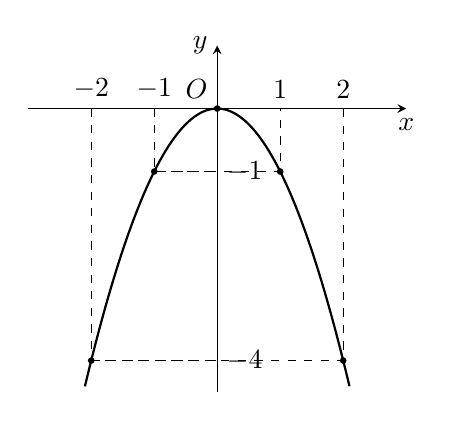
\begin{tikzpicture}[>=stealth,scale=0.8]
        \draw[->] (-3,0) -- (3,0) node[below] {$x$};
        \draw[->] (0,-4.5) -- (0,1) node[left] {$y$};
        \node[above left] at (0,0) {$O$};
        \draw[dashed] (-2,0) node[above] {$-2$} -- (-2,-4) -- (2,-4) -- (2,0) node[above] {$2$};
        \draw[dashed] (-1,0) node[above] {$-1$} -- (-1,-1) -- (1,-1) -- (1,0) node[above] {$1$};
        \draw[dashed] (-2,-4) -- (0,-4) node[right] {$-4$};
        \draw[dashed] (-1,-1) -- (0,-1) node[right] {$-1$};
        \draw[thick,smooth,samples=100,domain=-2.1:2.1] plot(\x,{-(\x)^2});
        \fill (-2,-4) circle (1.5pt) (-1,-1) circle (1.5pt) (0,0) circle (1.5pt) (1,-1) circle (1.5pt) (2,-4) circle (1.5pt);
    \end{tikzpicture}
    \end{center}
    \item Điểm $M$ thuộc $(P)$ có hoành độ gấp đôi tung độ nên $x = 2y \implies y = \dfrac{1}{2}x$.\\
    Ta có phương trình hoành độ giao điểm:
    $$-x^2 = \dfrac{1}{2}x \iff x^2 + \dfrac{1}{2}x = 0 \iff x\left(x + \dfrac{1}{2}\right) = 0 \iff \left[\begin{aligned} &x = 0\text{ (loại vì } M \ne O\text{)} \\ &x = -\dfrac{1}{2}\text{ (nhận)}. \end{aligned}\right.$$
    Với $x = -\dfrac{1}{2} \implies y = \dfrac{1}{2} \cdot \left(-\dfrac{1}{2}\right) = -\dfrac{1}{4}$.\\
    Vậy tọa độ điểm cần tìm là $M\left(-\dfrac{1}{2}; -\dfrac{1}{4}\right)$.
\end{enumerate}
}
\end{bt}

\begin{bt}%[9D6H20-2]
% nguon: Cụm 10 – Đề tham khảo Tuyển sinh 10 năm học 2026-2027 TP.HCM – Đề số 29
Cho phương trình $2x^2 - 3x - 5 = 0$.
\begin{enumerate}[a)]
    \item Chứng minh phương trình trên có hai nghiệm phân biệt $x_1, x_2$.
    \item Không giải phương trình, tính giá trị của biểu thức $A = x_1^2 + x_2^2 + 3x_1 x_2$.
\end{enumerate}
\loigiai{
\begin{enumerate}[a)]
    \item Phương trình $2x^2 - 3x - 5 = 0$ có $a = 2, b = -3, c = -5$.\\
    Ta có $\Delta = (-3)^2 - 4 \cdot 2 \cdot (-5) = 9 + 40 = 49 > 0$.\\
    Vì $\Delta > 0$ nên phương trình có hai nghiệm phân biệt $x_1, x_2$.
    \item Theo định lý Vi-ét, ta có:
    $$\begin{cases} x_1 + x_2 = \dfrac{3}{2} \\ x_1 x_2 = -\dfrac{5}{2}. \end{cases}$$
    Ta biến đổi biểu thức $A$:
    $$A = (x_1 + x_2)^2 + x_1 x_2.$$
    Thay $x_1 + x_2 = \dfrac{3}{2}$ và $x_1 x_2 = -\dfrac{5}{2}$ vào, ta được:
    $$A = \left(\dfrac{3}{2}\right)^2 + \left(-\dfrac{5}{2}\right) = \dfrac{9}{4} - \dfrac{10}{4} = -\dfrac{1}{4}.$$
\end{enumerate}
}
\end{bt}

\begin{bt}%[9D8H26-3]
% nguon: Cụm 10 – Đề tham khảo Tuyển sinh 10 năm học 2026-2027 TP.HCM – Đề số 29
Trong một chiếc hộp đựng các quả bóng cùng kích thước, cùng khối lượng và chất liệu, được đánh số lần lượt từ $1$ đến $10$. Lấy ngẫu nhiên một quả bóng từ trong hộp.
\begin{enumerate}[a)]
    \item Xác định không gian mẫu và số kết quả có thể xảy ra của phép thử.
    \item Tính xác suất của các biến cố sau:
    \begin{itemize}
        \item $A$: ``Số được ghi trên quả bóng lấy ra là số chẵn''.
        \item $B$: ``Số được ghi trên quả bóng lấy ra là số nguyên tố''.
    \end{itemize}
\end{enumerate}
\loigiai{
\begin{enumerate}[a)]
    \item Không gian mẫu của phép thử là:
    $$\Omega = \{1; 2; 3; 4; 5; 6; 7; 8; 9; 10\}.$$
    Số kết quả có thể xảy ra là $n(\Omega) = 10$.
    \item Tính xác suất của các biến cố:
    \begin{itemize}
        \item Các kết quả thuận lợi cho biến cố $A$ là các số chẵn: $\{2; 4; 6; 8; 10\}$.\\
        Số kết quả thuận lợi là $n(A) = 5$.\\
        Xác suất của biến cố $A$ là:
        $$P(A) = \dfrac{n(A)}{n(\Omega)} = \dfrac{5}{10} = \dfrac{1}{2}.$$
        \item Các kết quả thuận lợi cho biến cố $B$ là các số nguyên tố: $\{2; 3; 5; 7\}$.\\
        Số kết quả thuận lợi là $n(B) = 4$.\\
        Xác suất của biến cố $B$ là:
        $$P(B) = \dfrac{n(B)}{n(\Omega)} = \dfrac{4}{10} = \dfrac{2}{5}.$$
    \end{itemize}
\end{enumerate}
}
\end{bt}

\begin{bt}%[9H4V12-3]
% nguon: Cụm 10 – Đề tham khảo Tuyển sinh 10 năm học 2026-2027 TP.HCM – Đề số 29
Hai bạn Lâm và Dương rủ nhau đi câu cá bằng xe đạp từ nhà Lâm tại vị trí $A$ đến một hồ cá tại vị trí $B$. Trên đường đi, hai bạn phải vượt qua một con dốc có đỉnh ở vị trí $C$, chân đường vuông góc kẻ từ đỉnh dốc xuống mặt đất là $H$. Biết góc lên dốc là $\widehat{CAH} = 5^\circ$, góc xuống dốc là $\widehat{CBH} = 9^\circ$ và độ cao của con dốc là $CH = x\text{ (m)}$.
\begin{enumerate}[a)]
    \item Biểu diễn tổng quãng đường $S$ mà hai bạn đi từ $A$ đến $B$ theo $x$.
    \item Bạn Lâm đạp xe lên dốc với vận tốc $10\text{ km/h}$, mất $10$ phút thì đến đỉnh dốc, rồi từ đó thả dốc xuống với vận tốc $18\text{ km/h}$. Tính tổng thời gian hai bạn đi từ nhà đến hồ cá.
\end{enumerate}
\loigiai{
\begin{center}
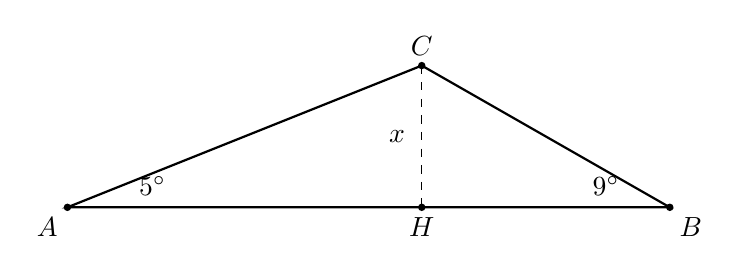
\begin{tikzpicture}[scale=0.9]
    \coordinate (H) at (0,0);
    \coordinate (C) at (0,2);
    \coordinate (A) at (-5,0);
    \coordinate (B) at (3.5,0);
    \draw[thick] (A) -- (C) -- (B) -- cycle;
    \draw[dashed] (C) -- (H);
    \node[below left] at (A) {$A$};
    \node[below right] at (B) {$B$};
    \node[above] at (C) {$C$};
    \node[below] at (H) {$H$};
    \node[left] at (-0.1,1) {$x$};
    \node at (-3.8,0.3) {$5^\circ$};
    \node at (2.6,0.3) {$9^\circ$};
    \fill (A) circle (1.5pt) (B) circle (1.5pt) (C) circle (1.5pt) (H) circle (1.5pt);
\end{tikzpicture}
\end{center}
\begin{enumerate}[a)]
    \item Trong tam giác vuông $AHC$ tại $H$:
    $$\sin A = \dfrac{CH}{AC} \implies AC = \dfrac{x}{\sin 5^\circ}\text{ (m)}.$$
    Trong tam giác vuông $BHC$ tại $H$:
    $$\sin B = \dfrac{CH}{BC} \implies BC = \dfrac{x}{\sin 9^\circ}\text{ (m)}.$$
    Tổng quãng đường $S$ hai bạn đi từ $A$ đến $B$ là:
    $$S = AC + BC = \dfrac{x}{\sin 5^\circ} + \dfrac{x}{\sin 9^\circ}\text{ (m)}.$$
    \item Đổi: $10\text{ phút} = \dfrac{1}{6}\text{ giờ}$.\\
    Chiều dài đoạn đường lên dốc $AC$ là:
    $$AC = v_1 \cdot t_1 = 10 \cdot \dfrac{1}{6} = \dfrac{5}{3}\text{ (km)}.$$
    Độ cao của con dốc là:
    $$CH = AC \cdot \sin 5^\circ = \dfrac{5}{3}\sin 5^\circ\text{ (km)}.$$
    Chiều dài đoạn đường xuống dốc $BC$ là:
    $$BC = \dfrac{CH}{\sin 9^\circ} = \dfrac{5\sin 5^\circ}{3\sin 9^\circ}\text{ (km)}.$$
    Thời gian hai bạn xuống dốc là:
    $$t_2 = \dfrac{BC}{v_2} = \dfrac{\dfrac{5\sin 5^\circ}{3\sin 9^\circ}}{18} = \dfrac{5\sin 5^\circ}{54\sin 9^\circ}\text{ (giờ)}.$$
    Tổng thời gian đi từ nhà đến hồ cá là:
    $$t = t_1 + t_2 = \dfrac{1}{6} + \dfrac{5\sin 5^\circ}{54\sin 9^\circ}\text{ (giờ)}.$$
    Đổi ra phút:
    $$t = \left(\dfrac{1}{6} + \dfrac{5\sin 5^\circ}{54\sin 9^\circ}\right) \cdot 60 = 10 + \dfrac{50\sin 5^\circ}{9\sin 9^\circ}\text{ (phút)} \approx 13{,}1\text{ phút (khoảng 13 phút 6 giây)}.$$
\end{enumerate}
}
\end{bt}

\begin{bt}%[9H0V31-3]
% nguon: Cụm 10 – Đề tham khảo Tuyển sinh 10 năm học 2026-2027 TP.HCM – Đề số 29
Tại một siêu thị có bán loại cam sành hình cầu có đường kính $8\text{ cm}$, vỏ dày $0{,}3\text{ cm}$. Khi ép, mỗi quả cam cho lượng nước ép bằng $88\%$ thể tích toàn bộ quả cam.
\begin{enumerate}[a)]
    \item Coi phần ruột cam cũng có dạng hình cầu đồng tâm với quả cam. Tính thể tích phần ruột của quả cam (kết quả làm tròn đến chữ số thập phân thứ hai).
    \item Bạn An cần chuẩn bị $6$ ly nước ép cam. Nước ép đựng trong các ly thủy tinh hình trụ có chiều cao lòng trong $15\text{ cm}$ và đường kính đáy lòng trong là $6\text{ cm}$. Mỗi ly chứa lượng nước cam bằng $70\%$ thể tích ly. Hỏi An cần ít nhất bao nhiêu quả cam để chuẩn bị đủ nước ép cho $6$ ly?
\end{enumerate}
Cho biết thể tích hình cầu là $V = \dfrac{4}{3}\pi R^3$ và thể tích hình trụ là $V = \pi R^2 h$.
\loigiai{
\begin{enumerate}[a)]
    \item Bán kính của quả cam là $R = 8 : 2 = 4\text{ (cm)}$.\\
    Bán kính của phần ruột cam là:
    $$r = 4 - 0{,}3 = 3{,}7\text{ (cm)}.$$
    Thể tích phần ruột cam là:
    $$V_{\text{ruột}} = \dfrac{4}{3}\pi r^3 = \dfrac{4}{3}\pi \cdot (3{,}7)^3 = \dfrac{50\,653\pi}{750} \approx 212{,}17\text{ (cm}^3\text{)}.$$
    \item Thể tích toàn bộ của một quả cam là:
    $$V_{\text{cam}} = \dfrac{4}{3}\pi \cdot 4^3 = \dfrac{256\pi}{3}\text{ (cm}^3\text{)}.$$
    Thể tích nước ép thu được từ một quả cam là:
    $$V_{\text{nước ép}} = 88\% \cdot V_{\text{cam}} = 0{,}88 \cdot \dfrac{256\pi}{3} = \dfrac{5\,632\pi}{75}\text{ (cm}^3\text{)}.$$
    Bán kính đáy của lòng ly thủy tinh là $R_{\text{ly}} = 6 : 2 = 3\text{ (cm)}$.\\
    Thể tích lòng một ly thủy tinh là:
    $$V_{\text{ly}} = \pi R_{\text{ly}}^2 h = \pi \cdot 3^2 \cdot 15 = 135\pi\text{ (cm}^3\text{)}.$$
    Lượng nước ép trong một ly là:
    $$70\% \cdot V_{\text{ly}} = 0{,}7 \cdot 135\pi = \dfrac{189\pi}{2}\text{ (cm}^3\text{)}.$$
    Tổng lượng nước ép cần chuẩn bị cho $6$ ly là:
    $$V_{\text{tổng}} = 6 \cdot \dfrac{189\pi}{2} = 567\pi\text{ (cm}^3\text{)}.$$
    Số quả cam cần dùng là:
    $$\dfrac{V_{\text{tổng}}}{V_{\text{nước ép}}} = \dfrac{567\pi}{\dfrac{5\,632\pi}{75}} = 567 \cdot \dfrac{75}{5\,632} \approx 7{,}55\text{ (quả)}.$$
    Vì số quả cam phải là số tự nhiên nên An cần ít nhất $8$ quả cam.
\end{enumerate}
}
\end{bt}

\begin{bt}%[9D6V21-3]
% nguon: Cụm 10 – Đề tham khảo Tuyển sinh 10 năm học 2026-2027 TP.HCM – Đề số 29
Ông Năm muốn dùng $100\text{ m}$ lưới để rào một khu đất hình chữ nhật sát bờ hồ thẳng để nuôi cá (không cần rào phần cạnh giáp bờ hồ). Để diện tích nuôi cá lớn nhất thì ông Năm nên rào khu đất với các kích thước như thế nào?
\loigiai{
Gọi $x\text{ (m)}$ là chiều rộng của phần đất rào (cạnh vuông góc với bờ hồ), điều kiện $0 < x < 50$.\\
Vì bờ hồ thẳng không cần rào lưới nên chiều dài của phần đất rào (cạnh song song với bờ hồ) là:
$$100 - 2x\text{ (m)}.$$
Diện tích phần đất nuôi cá là:
$$S = x(100 - 2x) = -2x^2 + 100x\text{ (m}^2\text{)}.$$
Ta biến đổi biểu thức $S$:
$$S = -2(x^2 - 50x) = -2(x^2 - 2 \cdot 25x + 25^2 - 25^2) = -2(x - 25)^2 + 1\,250.$$
Vì $(x - 25)^2 \ge 0$ với mọi $x$, nên $-2(x - 25)^2 \le 0 \implies S \le 1\,250$.\\
Dấu ``='' xảy ra khi $x - 25 = 0 \iff x = 25$ (thỏa mãn điều kiện).\\
Khi đó, chiều rộng là $25\text{ m}$ và chiều dài là $100 - 2 \cdot 25 = 50\text{ m}$.\\
Vậy để diện tích lớn nhất ($1\,250\text{ m}^2$), ông Năm nên rào hồ cá với chiều rộng $25\text{ m}$ và chiều dài $50\text{ m}$.
}
\end{bt}

\begin{bt}%[9H9C29-3]
% nguon: Cụm 10 – Đề tham khảo Tuyển sinh 10 năm học 2026-2027 TP.HCM – Đề số 29
Cho đường tròn tâm $O$ đường kính $BC$. Điểm $A$ nằm ngoài đường tròn sao cho tam giác $ABC$ nhọn ($\widehat{BAC} < 90^\circ$). Gọi $M, N$ lần lượt là giao điểm của $AB, AC$ với đường tròn $(O)$ ($M \ne B, N \ne C$). Hai đoạn thẳng $BN$ và $CM$ cắt nhau tại $I$.
\begin{enumerate}[a)]
    \item Chứng minh $AI \perp BC$ và tứ giác $AM I N$ nội tiếp một đường tròn.
    \item Gọi $D$ là điểm chính giữa của cung nhỏ $MN$. $BD$ cắt $CM$ tại $P$, $CD$ cắt $BN$ tại $Q$. Chứng minh rằng $DQ \cdot CD = BD \cdot DP$ và $\widehat{IPD} = \widehat{IQD}$.
    \item Giả sử $\widehat{BAC} = 60^\circ$ và $BC = 10\text{ cm}$. Tính độ dài đoạn thẳng $MN$ và chu vi đường tròn ngoại tiếp tam giác $MIN$.
\end{enumerate}
\loigiai{
\begin{center}
\begin{tikzpicture}[scale=0.95]
    \coordinate (B) at (-3,0);
    \coordinate (C) at (3,0);
    \coordinate (O) at (0,0);
    \def\R{3}
    \draw (O) circle (\R);
    \coordinate (A) at (0.5,4.5);
    \coordinate (M) at ($(A)!(C)!(B)$);
    \coordinate (N) at ($(A)!(B)!(C)$);
    \draw[thick] (A) -- (B) -- (C) -- cycle;
    \draw[thick] (B) -- (N);
    \draw[thick] (C) -- (M);
    \coordinate (I) at (intersection of B--N and C--M);
    \coordinate (H) at ($(B)!(A)!(C)$);
    \draw[dashed] (A) -- (H);
    \node[above] at (A) {$A$};
    \node[below left] at (B) {$B$};
    \node[below right] at (C) {$C$};
    \node[below] at (O) {$O$};
    \node[above left] at (M) {$M$};
    \node[above right] at (N) {$N$};
    \node[below] at (I) {$I$};
    \node[below] at (H) {$H$};
    \fill (A) circle (1.5pt) (B) circle (1.5pt) (C) circle (1.5pt) (M) circle (1.5pt) (N) circle (1.5pt) (I) circle (1.5pt) (H) circle (1.5pt);
\end{tikzpicture}
\end{center}
\begin{enumerate}[a)]
    \item Ta có $\widehat{BMC} = 90^\circ$ và $\widehat{BNC} = 90^\circ$ (các góc nội tiếp chắn nửa đường tròn đường kính $BC$).\\
    Suy ra $CM \perp AB$ và $BN \perp AC$.\\
    Trong tam giác $ABC$, hai đường cao $BN$ và $CM$ cắt nhau tại $I$, do đó $I$ là trực tâm của tam giác $ABC$.\\
    Suy ra $AI \perp BC$.\\
    Tứ giác $AM I N$ có $\widehat{AM I} = \widehat{AN I} = 90^\circ$, nên $\widehat{AM I} + \widehat{AN I} = 180^\circ$.\\
    Do đó tứ giác $AM I N$ nội tiếp đường tròn đường kính $AI$.
    \item Vì $D$ là điểm chính giữa của cung nhỏ $MN$ nên số đo cung $DM$ bằng số đo cung $DN$.\\
    Suy ra $\widehat{DBM} = \widehat{DCN}$ (hai góc nội tiếp chắn hai cung bằng nhau).\\
    Xét $\triangle PBM$ và $\triangle QCN$ có:
    $$\widehat{PMB} = \widehat{QNC} = 90^\circ, \quad \widehat{PBM} = \widehat{QCN}.$$
    Suy ra $\triangle PBM \backsim \triangle QCN$ (g-g) $\implies \widehat{BPM} = \widehat{CQN}$.\\
    Mà $\widehat{DPC} = \widehat{BPM}$ và $\widehat{DQB} = \widehat{CQN}$ (các cặp góc đối đỉnh), nên $\widehat{DPC} = \widehat{DQB}$.\\
    Xét $\triangle DPC$ và $\triangle DQB$ có:
    $$\widehat{BDC}\text{ chung, } \widehat{DPC} = \widehat{DQB}.$$
    Suy ra $\triangle DPC \backsim \triangle DQB$ (g-g) $\implies \dfrac{DP}{DQ} = \dfrac{DC}{DB} \implies DQ \cdot CD = BD \cdot DP$.\\
    Từ $\triangle DPC \backsim \triangle DQB$ ta có $\widehat{DPC} = \widehat{DQB}$, suy ra $\widehat{IPD} = \widehat{IQD}$.
    \item Xét $\triangle AMN$ và $\triangle ACB$ có:
    $$\widehat{BAC}\text{ chung, } \widehat{AMN} = \widehat{ACB}\text{ (cùng bù với góc } \widehat{BMN}\text{)}.$$
    Suy ra $\triangle AMN \backsim \triangle ACB$ (g-g) $\implies \dfrac{MN}{BC} = \dfrac{AM}{AC}$.\\
    Trong tam giác vuông $AMC$, ta có $\dfrac{AM}{AC} = \cos \widehat{BAC} = \cos 60^\circ = \dfrac{1}{2}$.\\
    Do đó:
    $$MN = \dfrac{1}{2}BC = \dfrac{1}{2} \cdot 10 = 5\text{ (cm)}.$$
    Vì tứ giác $AM I N$ nội tiếp đường tròn đường kính $AI$ nên đường tròn ngoại tiếp tam giác $MIN$ cũng chính là đường tròn đường kính $AI$.\\
    Xét $\triangle AMI$ và $\triangle CMB$ có:
    $$\widehat{AMI} = \widehat{CMB} = 90^\circ, \quad \widehat{MAI} = \widehat{MCB}\text{ (cùng phụ } \widehat{ABC}\text{)}.$$
    Suy ra $\triangle AMI \backsim \triangle CMB$ (g-g) $\implies \dfrac{AI}{BC} = \dfrac{AM}{CM}$.\\
    Trong tam giác vuông $AMC$, ta có $\dfrac{AM}{CM} = \cot \widehat{BAC} = \cot 60^\circ = \dfrac{\sqrt{3}}{3}$.\\
    Suy ra:
    $$AI = BC \cdot \dfrac{\sqrt{3}}{3} = 10 \cdot \dfrac{\sqrt{3}}{3} = \dfrac{10\sqrt{3}}{3}\text{ (cm)}.$$
    Chu vi của đường tròn ngoại tiếp tam giác $MIN$ là:
    $$C = \pi \cdot AI = \pi \cdot \dfrac{10\sqrt{3}}{3} = \dfrac{10\pi\sqrt{3}}{3}\text{ (cm)}.$$
\end{enumerate}
}
\end{bt}
